\chapter{پیشنیاز های نصب و معرفی قسمت های مختلف}\label{ch:req}

\section{نرم‌افزار‌های کلی}
در این پروژه از جهت آنکه نسخه قبلی و پیشینی برای  آن نبوده است، به ناچار می‌بایست که کد آن از صفر تا صد آن به صورت دستی نوشته شود. از این‌رو، پیچیدگی های بسیار فراوان را به طور خاص در پی داشت. ابزار های زیادی نیز بنابه شرایط در آن استفاده شد که ارتباط بین آن ابزار ها و اجزا، بر این پیچیدگی پیاده سازی طرح افزوده بود.

ابزار های اصلی و کلی که در این پروژه استفاده شده بود، عبارتند از:

\begin{itemize}
	\item 
	\textbf{نرم افزار 
	\glspl{w:prescan}}
	، نسخه \lr{$8.5.0$}
	
	\item 
	\textbf{نرم افزار 
	\glspl{w:matlab}	
}
	، نسخه \lr{R2017b}
	\item 
	\textbf{زبان برنامه نویسی پایتون}
	، نسخه \lr{$3.6.9$}
\end{itemize}

بنابراین برای راه اندازی مجدد کد این پروژه لازم است که موارد بالا روی کامپیوتر شخص به صورت کامل نصب باشد.

همچنین لازم به ذکر است که برخی ابزارات دیگر نیز در این پروژه استفاده شده است که احتمالا با نصب موارد بالا دیگر نیازی به نصب آن ها به صورت جداگانه نیست. هدف این ابزار ها ایجاد اتصال بین اجزای اصلی گفته شده است. این گروه شامل موارد زیر هستند:

\begin{itemize}
	\item 
	\textbf{\glspl{w:simulink}}
	، جهت اتصال بین متلب و پری اسکن
	
	\item 
	\textbf{شبکه \lr{UDP}}
	\RTLfootnote{برای این منظور از ماژول \lr{socket} در پایتون استفاده شده است. }
	، جهت اتصال داده های پویا 
	\LTRfootnote{Dynamic Data}
	بین پایتون و سیمولینک
	
	\item \textbf{\glspl{w:matlabengine}}
	، جهت اتصال داده های ساکن
	\LTRfootnote{Static Data}
	بین پایتون و سیمولینک
\end{itemize}

در این فصل جزئیات بیشتری در مورد لزوم و دلیل استفاده از این ابزار ها بررسی می‌شود.




\section{پیشنیاز های پایتون}

\begin{note}

کد پایتون در این پروژه شامل دو قسمت کلی زیر می‌شود. این دو دسته در شکل
\ref{fig:python-layers-env-alg}
مشخص هستند.
\begin{enumerate}
	\item 
	دسته اول مربوط به آن بخش از پروژه است که وظیفه اصلی آن ارتباط پیدا کردن با محیط متلب و پری اسکن و ایجاد یک نوع واسط کاربری است. گرفتن و فرستادن اطلاعات مخصوص این قسمت است.
	\item 
	دسته دوم با محیط و نحوه ارتباط آن کاری ندارد و تمرکز خود را بر‌روی الگوریتم خود که در این جا از الگوریتم های یادگیری تقویتی استفاده شده است، قرار داده است.
\end{enumerate}

\end{note}

\begin{figure}
	\centering
	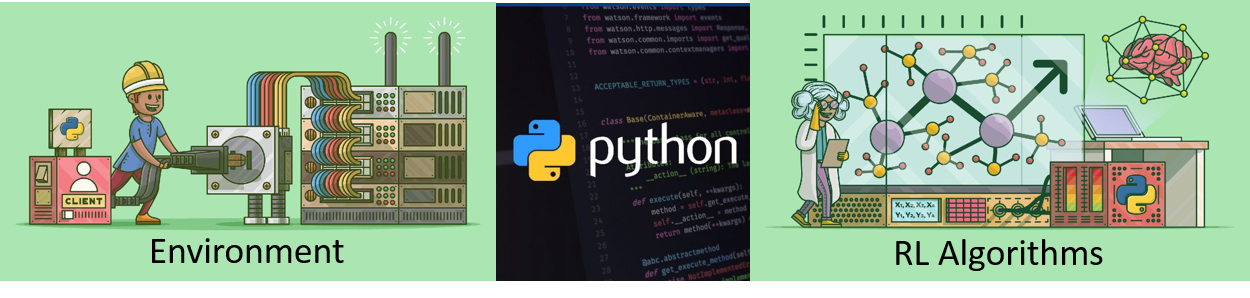
\includegraphics[width=\linewidth]{Figures/python-layers-env-alg}
	\caption{تقسیم بندی وظایف اصلی کد پایتون}
	\label{fig:python-layers-env-alg}
\end{figure}


دسته اول (سمت چپ تصویر
\ref{fig:python-layers-env-alg}
)
به پکیج های زیر احتیاج دارد:
\begin{multicols}{3}
\begin{itemize}
	\item \lr{numpy} \item \lr{socket} \item\lr{time} \item \lr{os}
	\item \lr{matlab.engine} \item \lr{gym}
\end{itemize}
\end{multicols}
اگر از 
\glspl{w:anaconda}
برای پایتون استفاده می‌کنید غیراز دو بسته 
\lr{gym}
و 
\lr{matlab.engine}
به صورت پیش‌فرض نصب شده اند در صورت عدم نصب آن ها را با استفاده از 
\lr{pip}\RTLfootnote{مثلا بسته \lr{numpy} را با استفاده از دستور \lr{\texttt{pip install numpy}} نصب می‌توان کرد.}
می‌توان نصب کرد.

بسته \lr{gym} که در این فصل به‌تفصیل در مورد آن بحث شده است، به راحتی با همان دستور \texttt{pip} نصب می‌شود. اما نصب 
\lr{matlab.engine}
یا همان
\glspl{w:matlabengine}
متفاوت است و نمی‌توان آن را نیز به همان روش نصب کرد.

دسته دوم شامل بسته های زیر است:
\begin{itemize}
	\item \lr{gym[atari]} یا \lr{gym[all]}
	\item \lr{tensorflow}
	\item \lr{stable-baseline}
	
\end{itemize}

این بسته ها در لایه الگوریتم استفاده شده است.(در مورد این لایه در فصل 
\ref{ch:alg}
بیشتر صحبت خواهد شد.)
هر سه‌تای این بسته ها با همان دستور \lr{pip} به راحتی نصب می‌شوند.





